% =====================================================================
%  Prabhavit Gupta, one-page CV (Marsh - Software Engineer Python)
%  Compile:  tectonic main_Marsh_SoftwareEngineer.tex
%  Needs:    photo.jpg in the same folder as this .tex
%  Rules:    ONE PAGE. No em-dashes. Plain voice. Clickable companies.
%            No "sample of my code" line. Salary blank or "negotiable".
%            Never write "no-code" or "Bubble", say "off a legacy stack".
% =====================================================================
\documentclass[a4paper,10pt]{article}

\usepackage[T1]{fontenc}
\usepackage[utf8]{inputenc}
\usepackage[top=0.75cm,bottom=0.75cm,left=1.0cm,right=1.0cm]{geometry}
\usepackage{titlesec}
\usepackage{enumitem}
\usepackage{hyperref}
\usepackage{xcolor}
\usepackage{graphicx}

\definecolor{accent}{HTML}{1F4E78}
\hypersetup{colorlinks=true, urlcolor=accent, linkcolor=accent}
\pagestyle{empty}
\setlength{\parindent}{0pt}

\titleformat{\section}{\large\bfseries\color{accent}}{}{0em}{}[\vspace{-0.6em}\rule{\textwidth}{0.8pt}]
\titlespacing{\section}{0pt}{2pt}{1pt}

\newcommand{\role}[4]{%
 \textbf{#1} \hfill \textbf{#2}\\[1pt]%
 \textit{#3} \hfill \textit{#4}\\[2pt]%
}
\setlist[itemize]{leftmargin=1.2em, itemsep=0pt, topsep=1pt, parsep=0pt}

\begin{document}

% ================= HEADER =================
\begin{minipage}[c]{0.80\textwidth}
 {\Huge\bfseries Prabhavit Gupta}\\[3pt]
 {\color{accent}\large Software Engineer}\\[6pt]
 {\footnotesize +39 351 610 7807 ~$\vert$~
 \href{mailto:prabhavitg@gmail.com}{prabhavitg@gmail.com} ~$\vert$~
 \href{https://www.linkedin.com/in/prabhavit/}{linkedin.com/in/prabhavit} ~$\vert$~
 \href{https://github.com/prab-gupta}{github.com/prab-gupta} ~$\vert$~
 Venice, Italy}
\end{minipage}\hfill
\begin{minipage}[c]{0.18\textwidth}
 \raggedleft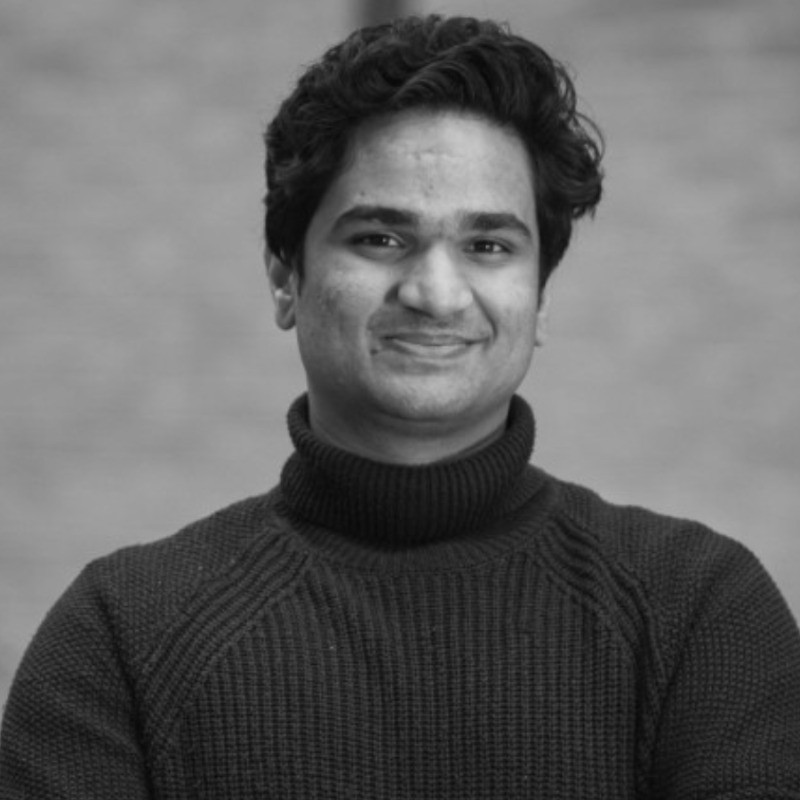
\includegraphics[width=2.0cm]{photo.jpg}
\end{minipage}
\vspace{-2pt}

% ================= SUMMARY =================
\section{Summary}
Software engineer who ships production web applications and the AI features on top of them. At FlowSpace, owned platform architecture, migrated a live marketplace off a legacy stack to Next.js and Laravel (scaling to 4,500+ users), built an automated ingestion pipeline with human-in-the-loop review (900+ listings drafted), and deployed live support agents. Daily stack: TypeScript, Next.js, Python, PostgreSQL, Docker, and Claude Code.

% ================= SKILLS =================
\section{Skills}
\begin{itemize}
 \item \textbf{Enablement \& Developer Platforms:} Internal developer tooling, reproducible environments, CI/CD automation, Claude Code agentic workflows, repository standards, testing automation, n8n, human-in-the-loop review
 \item \textbf{Product Engineering \& Full Stack:} Python, TypeScript, JavaScript, Next.js, Node.js, Laravel (PHP), PostgreSQL, Supabase, responsive UI, state management, REST APIs, webhooks, schema validation
 \item \textbf{Infrastructure \& Reliability:} Docker, containerized deployments, cloud infrastructure (AWS, GCP), Playwright, automated QA, API contracts, complexity management, technical debt containment
\end{itemize}

% ================= EXPERIENCE =================
\section{Experience}

\role{\href{https://flowspace.co}{FlowSpace.co}}{Mar 2024 - Aug 2026}{Lead Developer (Full-time, Freelance)}{London, UK (remote)}
\begin{itemize}
 \item Migrated a live marketplace off a legacy stack to coded Next.js and Laravel, establishing clean API abstractions, repository standards, and scaling from 2,000 to 4,500+ active users.
 \item Built an AI ingestion pipeline (n8n, Claude API, TypeScript) parsing unstructured brochures (PDF, spreadsheets, web) into structured listings with human-in-the-loop review; 900+ listings drafted.
 \item Deployed support agents that answer user queries against live platform records, with confidence-based escalation to human operators.
 \item Integrated OfficeRnD and Nexudus APIs for automated bookings, and built CRM and GTM automations for lead routing and outbound sync.
\end{itemize}

\role{\href{https://get2germany.com}{Get2Germany.com}}{Jan 2024 - May 2024}{Developer \& Automation Specialist (Part-time)}{Berlin, Germany}
Integrated Google APIs, built AI automation tools in n8n for data extraction and cataloging, and optimized relational database queries.\\[1pt]

\role{\href{https://clubee.com}{Clubee.com}}{Sep 2023 - Aug 2024}{Developer \& QA (Full-time, Freelance)}{Foetz, Luxembourg}
Integrated the Clubee API across the frontend, developed federation-dashboard tools, and established unit testing and QA suites.\\[1pt]

\role{\href{https://tractionboard.co}{Tractionboard.co}}{Aug 2023 - Oct 2023}{Developer (Internship)}{Utrecht, Netherlands}
Integrated OpenAI and Sendgrid APIs, built responsive frontend interfaces, and implemented automated error tracking.

% ================= FREELANCE PROJECTS =================
\section{Freelance Projects}
\begin{itemize}
 \item \textbf{\href{https://smarturlink.com/}{Urlink}} (2025), Project Manager \& AI-Assisted Developer. Built platform architecture and client logic with Next.js, Supabase, and Netlify; automated continuous integration and delivery.
 \item \textbf{\href{https://ultrastrategy.com}{UltraStrategy}} (2024 to 2025), AI Automation Developer. Built an automated CV-parsing tool (LLM data extraction) with n8n and Eden AI, delivering structured JSON schemas.
 \item \textbf{\href{https://www.qomodo.me/}{Qomodo}} (2024 to 2025), AI Developer. Built branch management dashboards from Figma designs, implementing modular UI components and state handling.
\end{itemize}

% ================= CERTIFICATIONS =================
\section{Certifications}
Microsoft Copilot Studio Agent Academy \textbullet\ Microsoft: Introduction to building AI agents \textbullet\ Microsoft Power Automate \textbullet\ Tray.AI Build Practitioner (Sep 2024)

% ================= EDUCATION =================
\section{Education}
\textbf{Ca' Foscari University of Venice} \hfill Oct 2020 - Jun 2024\\
BA Philosophy, International Studies \& Economics (Minor: Entrepreneurship)

% ================= AUTH =================
\vspace{2pt}
{\small \textbf{Work authorization:} European Long Term Residence Permit (Italy); available immediately. \quad \textbf{Languages:} Hindi (native), English (fluent C2), Italian (conversational).}

\end{document}
